\documentclass{beamer}

\mode<presentation>
{
  \usetheme{Madrid}
  \usecolortheme{default}
  \usefonttheme{default}
  \setbeamertemplate{caption}[numbered]
}

\usepackage{CJKutf8}
\usepackage[USenglish]{babel}
\usepackage[utf8]{inputenc}
\usepackage{ragged2e}
\usepackage{booktabs}
\usepackage{array}

\title[Analysis of Political Activities on SNS]{社群網站上之政治活動分析}
\subtitle{以台灣 2016 年總統選舉為例}
\author[Yu Wen Pwu]{蒲郁文}
\institute[NCTU]{國立交通大學資訊工程學系}
\date[Undergraduate Research]{106A 學士班專題競賽}

\AtBeginSection[]
{
  \begin{frame}{研究問題}
    \tableofcontents[currentsection]
  \end{frame}
}

\newcolumntype{L}[1]{>{\raggedright\arraybackslash}p{#1}}
\newcolumntype{C}[1]{>{\centering\arraybackslash}p{#1}}
\newcolumntype{R}[1]{>{\raggedleft\arraybackslash}p{#1}}

\begin{document}
\begin{CJK}{UTF8}{bkai}

\begin{frame}
  \titlepage
\end{frame}

\begin{frame}
\begin{block}{摘要}
\justifying
\qquad 本研究嘗試使用關鍵字擷取(keyword extraction)、%
情感分析(sentiment analysis)、社會網絡分析(social network analysis)等方法,%
分析 2016 年台灣總統選舉競選期間臉書各大政治性粉絲專頁之公開資料,探討使用者於社群網站上之政治活動的模式。%
本研究發現此次選舉有 26.63\% 的社群媒體貼文是攻擊型競選,與台灣、中國或中國國民黨有關的議題是人們最關注的焦點,%
且特定族群會傾向於分享特定來源的資訊。%
同時,本研究也提供了後續研究者一套有效地自動化分析線上政治活動的方法。%
\vskip 1em
關鍵字\enskip---\enskip社群媒體、自動化內容分析、社會網絡分析、數位行動主義、政治參與%
\end{block}
\end{frame}

\begin{frame}{研究問題}
  \tableofcontents
\end{frame}

\begin{frame}{資料蒐集}
\begin{itemize}
\item 資料集:2016 年台灣總統選舉競選期間臉書各大政治性粉絲專頁之公開資料
\item 時間範圍:投票日前三個月至投票日止
\item 資料總數:18,967 筆臉書貼文,來自 135 個台灣熱門的政治性粉\\絲專頁
\item 蒐集方法:
  \begin{itemize}
  \item 使用 Facebook Graph API
  \item 參考 Socialbakers 及 Likeboy 提供之社群媒體統計數據,輔以我個\\人的自身經驗,決定欲蒐集的粉絲專頁清單
  \item 查詢這些粉絲專頁最新的按讚數,只保留擁有超過一萬個讚的粉絲專頁
  \end{itemize}
\end{itemize}
\end{frame}

\begin{frame}{斷詞}
\begin{itemize}
\item 採用中央研究院資訊科學研究所中文詞知識庫小組所研發之\\中文斷詞系統
  \begin{itemize}
  \item 對台灣本地的文本有較好的表現
  \item 具有良好的未知詞辨識能力
  \end{itemize}
\item 斷詞前先對貼文進行預處理
\item 使用物件關係對映與資料庫存放資料
\end{itemize}
\end{frame}

\section{
各政黨/侯選人/意見領袖分別發佈了多少篇貼文?\texorpdfstring{\protect\\}{}
\hspace{.35em}每日的貼文數量隨著時間有什麼樣的改變?
}

\begin{frame}{總體分佈}
\begin{itemize}
\item 使用 pandas、Matplotlib、Plotly 等函式庫
\item 繪製貼文數量對時間的關係圖
\item 繪製累計貼文數量對時間的關係圖
\item 統計各粉絲專頁分別有多少筆貼文、佔全部貼文的百分比
\end{itemize}
\end{frame}

\begin{frame}{總體分佈}
\begin{columns}
\begin{column}{.68\textwidth}
  \begin{figure}
    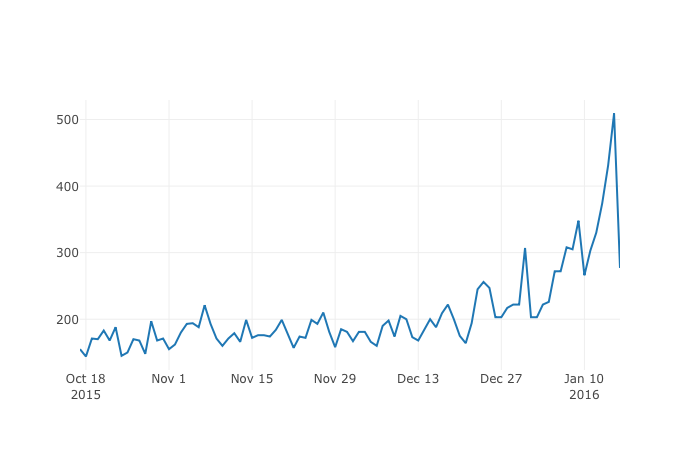
\includegraphics[width=\textwidth, height=\textheight, keepaspectratio]{quantity_time_graph_ng}
    \caption{貼文數量對時間的關係圖}
  \end{figure}
\end{column}
\begin{column}{.28\textwidth}
  \qquad 貼文數量呈現週期性變化,每逢假日貼文數量就會顯著降低。%
  隨著投票日的接近,各政黨/侯選人/意見領袖也愈來愈踴躍地在社群網站上發佈貼文。%
\end{column}
\end{columns}
\end{frame}

\begin{frame}{總體分佈}
\begin{figure}
  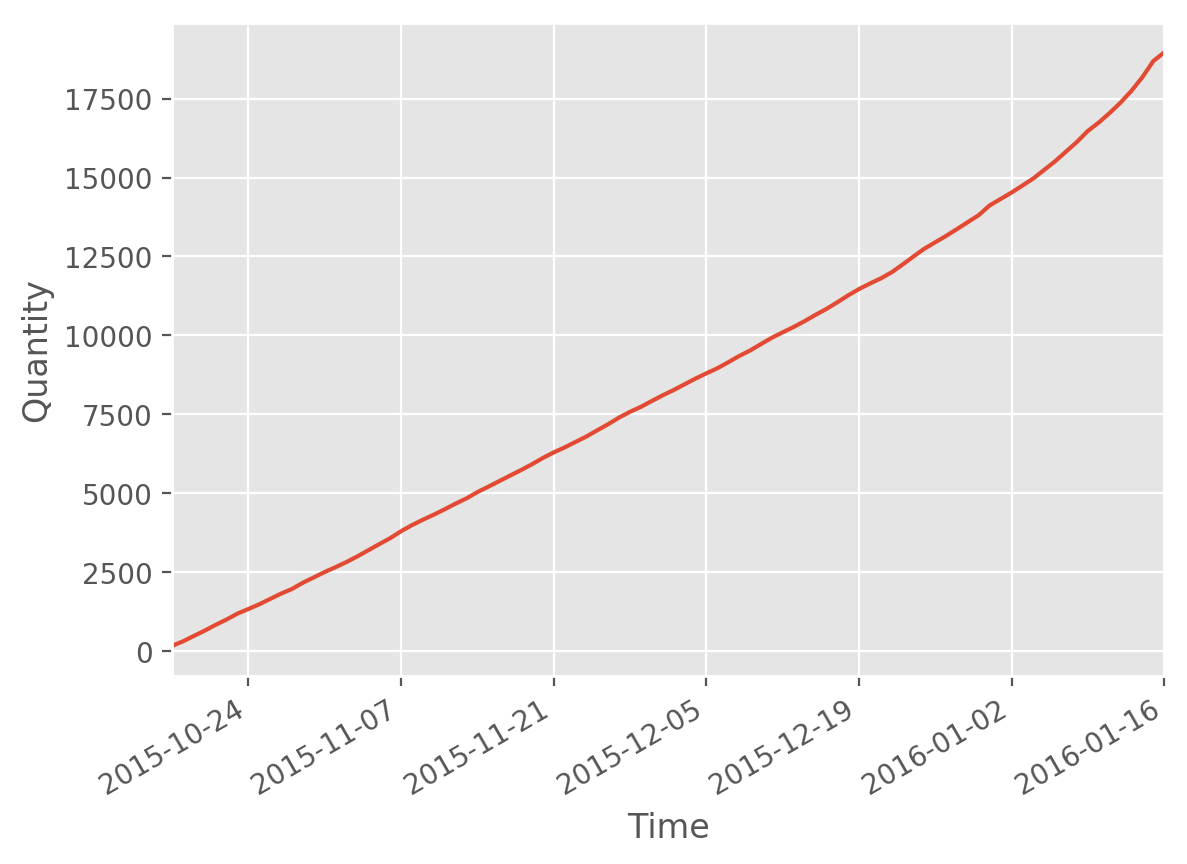
\includegraphics[width=.7\textwidth, height=.7\textheight, keepaspectratio]{quantity_time_cumulative_graph}
  \caption{累計貼文數量對時間的關係圖}
\end{figure}
\end{frame}

\begin{frame}{總體分佈}
\begin{table}
\caption{各粉絲專頁的貼文數量(節錄)}
\begin{tabular}{@{}L{10em}C{4em}C{4em}@{}}
  \toprule
  粉絲專頁名稱 & 貼文數量 & 百分比 \\
  \midrule
  柯建銘 & 485 & 2.56\% \\
  Taiwan Fugue & 361 & 1.90\% \\
  台灣新力量/羅致政\dots & 337 & 1.78\% \\
  宋楚瑜找朋友 & 334 & 1.76\% \\
  反馬英九聯盟 & 330 & 1.74\% \\
  林昶佐 Freddy Lim & 320 & 1.69\% \\
  基進黨(基進側翼) & 319 & 1.68\% \\
  BillyPan 潘建志醫師 & 306 & 1.61\% \\
  宋楚瑜 & 301 & 1.59\% \\
  綠黨 & 297 & 1.57\% \\
  民主進步黨 & 293 & 1.54\% \\
  \bottomrule
\end{tabular}
\end{table}
\end{frame}

\section{
各政黨/侯選人/意見領袖最關心的議題是什麼?\texorpdfstring{\protect\\}{}
\hspace{.35em}人們關注的焦點隨著時間有什麼樣的改變?\texorpdfstring{\protect\\}{}
\hspace{.35em}本次選舉人們最關心什麼?
}

\begin{frame}{關鍵字擷取}
\begin{itemize}
\item 使用 SnowNLP 函式庫實作的 TextRank 演算法
  \begin{itemize}
  \item 衍生自 PageRank 演算法
  \item 不需輸入全部文本 (cf. tf--idf)
  \end{itemize}
\item 改良 SnowNLP 函式庫提供的停用字清單
\item 合併範圍內的貼文進行分析
\item 分析各粉絲專頁發佈的貼文的關鍵字
\item 分析各時間區間發佈的貼文的關鍵字
\item 分析整個競選期間所有人發佈的貼文的關鍵字
\end{itemize}
\end{frame}

\begin{frame}{關鍵字擷取}
\begin{columns}
\begin{column}{.64\textwidth}
  \begin{table}
  \caption{依作者劃分(節錄)}
  \begin{tabular}{@{}L{8em}ll@{}}
    \toprule
    粉絲專頁名稱 & \#1 & \#2 \\
    \midrule
    朱立倫 & 台灣 & 新 \\
    大安推范雲 & 范雲 & 台灣 \\
    王丹网站 Wa\dots & 中國 & 中 \\
    國民黨青年團 & 青年 & 台灣 \\
    呂欣潔 Jennif\dots & 政治 & 欣潔 \\
    管碧玲 (kuan\dots & 管媽 & 市長 \\
    段宜康 & 朱立倫 & 國民黨 \\
    鄉民實業坊 & 黑子 & 種 \\
    我是台灣人 (\dots & 台灣 & 綠黨 \\
    林智堅 & 新竹市 & 新竹 \\
    BillyPan 潘\dots & 醫師 & 台灣 \\
    \bottomrule
  \end{tabular}
  \end{table}
\end{column}
\begin{column}{.31\textwidth}
  \qquad 從此表我們可以看出各政黨/侯選人/意見領袖重視的議題。%
  例如,中國國民黨關注朱立倫以及經濟、兩岸等事務;王金平關注國會、改革等事務;%
  綠黨關注勞工、環境等議題;而馬躍.比吼則關注原住民的文化和土地等等。%
\end{column}
\end{columns}
\end{frame}

\begin{frame}{關鍵字擷取}
\begin{columns}
\begin{column}{.64\textwidth}
  \begin{table}
  \caption{依時間劃分(節錄)}
  \begin{tabular}{@{}L{7.5em}ll@{}}
    \toprule
    時間區間 & \#1 & \#3 \\
    \midrule
    11/15 $\sim$ 11/22 & 台灣 & 政府 \\
    11/08 $\sim$ 11/15 & 台灣 & 中國 \\
    11/01 $\sim$ 11/08 & 台灣 & 中國 \\
    10/25 $\sim$ 11/01 & 台灣 & 國民黨 \\
    10/17 $\sim$ 10/25 & 台灣 & 新 \\
    \bottomrule
  \end{tabular}
  \end{table}
\end{column}
\begin{column}{.31\textwidth}
  \qquad 透過此表,我們可以發現人們關注的焦點皆圍繞在台灣、中國、國民黨上,唯有在 11 月 1 日至 11 月 8 日間,%
  由於舉行兩岸領導人會面,馬英九、馬習會也躍升為社群網站上的討論焦點。%
\end{column}
\end{columns}
\end{frame}

\begin{frame}{關鍵字擷取}
\begin{columns}
\begin{column}{.64\textwidth}
  \begin{table}
  \caption{合併所有貼文(節錄)}
  \begin{tabular}{@{}lll@{}}
    \toprule
    \#1 & \#3 & \#7 \\
    \midrule
    台灣  & 國民黨 & 中國  \\
    \bottomrule
  \end{tabular}
  \end{table}
\end{column}
\begin{column}{.31\textwidth}
  \qquad 此表告訴我們本次選舉人們最關心跟台灣和中國有關的議題,而國民黨也是人們討論的焦點。%
  值得一提的是,此次選舉的另一大黨,民主進步黨,並未出現在前十大關鍵字之中。%
\end{column}
\end{columns}
\end{frame}

\section{
哪些政黨/候選人/意見領袖最常使用攻擊型競選?\texorpdfstring{\protect\\}{}
\hspace{.35em}什麼時候人們最常使用攻擊型競選?\texorpdfstring{\protect\\}{}
\hspace{.35em}本次選舉有多少比例的貼文是攻擊型競選?
}

\begin{frame}{情感分析}
\begin{itemize}
\item 將全部貼文分為兩個類別
  \begin{itemize}
  \item 攻擊型競選:貼文內容是以批評反對陣營為主、貼文重點是在批評反對陣營
  \item 說服型競選:非屬攻擊型競選的貼文(包含中立貼文)
  \end{itemize}
\item 分析每筆貼文的情感,再進行統計
\item 自行實作單純貝氏分類器
  \begin{itemize}
  \item 二元化多項單純貝氏(binarized multinomial naive Bayes)模型
  \item 只管一個單詞在一篇文章中有沒有出現,不管該單詞在文中究竟出現了多少遍
  \end{itemize}
\item 均勻地選取 948 筆(約5%)貼文作為訓練與測試資料,人工標\\記情感類型
\item 使用十等分交叉測試來評估模型的表現
\end{itemize}
\end{frame}

\begin{frame}{情感分析}
\begin{columns}
\begin{column}{.55\textwidth}
  \begin{figure}
    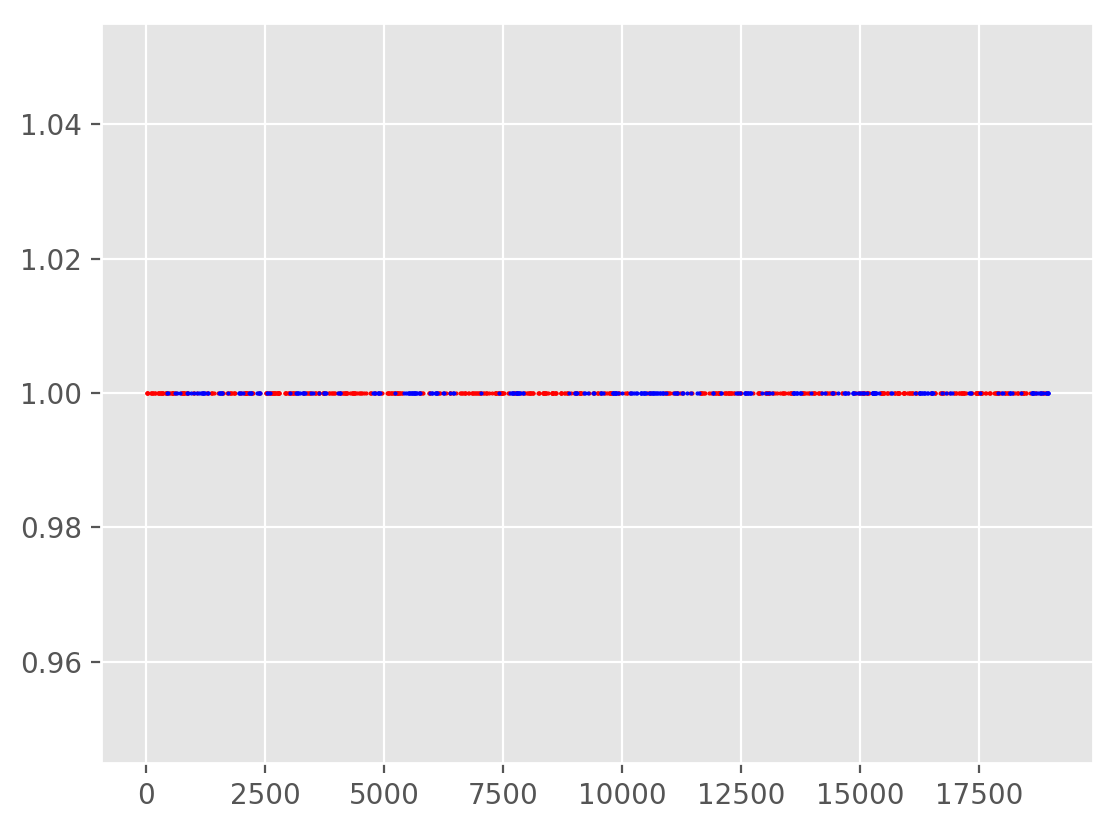
\includegraphics[width=\textwidth, height=\textheight, keepaspectratio]{meta}
    \caption{訓練/測試貼文的分佈圖}
  \end{figure}
\end{column}
\begin{column}{.40\textwidth}
  \qquad 圖中的每個點皆代表一筆訓練/測試貼文,點的水平位置代表它在所有貼文中的位置。%
  紅點代表說服型競選貼文,一共有 651 筆;藍點代表攻擊型競選貼文,一共有 297 筆。\par
  \qquad 本情感分類模型的準確度(accuracy)為 86.82\%,查準率(precision)為 87.6 5\%,%
  查全率(recall)為 87 .65\%,F 度量(F-measure)為 87.65\%。%
\end{column}
\end{columns}
\end{frame}

\begin{frame}{情感分析}
\begin{table}
\caption{貼文情感分析(節錄)}
\begin{tabular}{@{}L{7.2em}R{4em}R{4em}R{1em}R{4em}R{5em}@{}}
  \toprule
   \newline粉絲專頁名稱\newline  & %
   \enspace01/10\newline\hspace*{1.35em}$\vert$\newline01/17 & %
   \enspace01/03\newline\hspace*{1.35em}$\vert$\newline01/10 & %
   \newline\,$\ldots$\newline  & %
   \enspace10/17\newline\hspace*{1.35em}$\vert$\newline10/25 & %
   {\bfseries  所有  時間  區間} \\
  \midrule
  朱立倫 & 1/30 & 1/18 & $\ldots$ & 1/5 & 10/210 \\
  大安推范雲 & 2/35 & 0/27 & $\ldots$ & 1/13 & 14/239 \\
  王丹网站 Wa\dots & 3/14 & 6/11 & $\ldots$ & 5/12 & 37/137 \\
  國民黨青年團 & 1/4 & 0/4 & $\ldots$ & 0/0 & 4/51 \\
  $\,\vdots$ & $\vdots$ & $\vdots$ & $\ddots$ & $\vdots$ & $\vdots$ \\
  宋楚瑜 & 7/57 & 4/51 & $\ldots$ & 1/22 & 32/294 \\
  特急件小周\dots & 19/25 & 13/20 & $\ldots$ & 4/6 & 99/142 \\
  {\bfseries 所有粉絲專頁} & 509/2355 & 446/1868 & $\ldots$ & 336/1275 & 4827/18128 \\
  \bottomrule
\end{tabular}
\end{table}
\end{frame}

\begin{frame}{情感分析}
\justifying
\qquad 此次選舉只有 26.63\% 的社群媒體貼文是攻擊型競選。%
許多政治人物都不常使用攻擊型競選,然而,具鮮明政治立場,或以抨擊反對陣營為目的的意見領袖,則較常使用攻擊型競選。%
Taiwan Fugue、反馬英九聯盟、不禮貌鄉民團、藍白拖的逆襲等粉絲專頁攻擊型競選貼文的比例皆超過八成。%
這也有可能是政治人物為了營造正面競選的形象所進行的分工。\par
\qquad 使用攻擊型競選的比例並未隨著時間而有太大的變化,唯有在 11 月 1 日至 11 月 8 日間,%
或許是因為舉行兩岸領導人會面的緣故,攻擊型競選貼文的比例比平時高出了一成左右。%
另外,在投票日前一週,使用攻擊型競選的比例則比平時低了 5\% 左右。%
\end{frame}

\section{
各發文者與其分享的資訊的來源有什麼樣的關係?\texorpdfstring{\protect\\}{}
\hspace{.35em}特定族群是否會傾向於分享特定來源的資訊?
}

\begin{frame}{社會互動}
\begin{itemize}
\item 探討社群網站上的「分享」網絡
\item 資料預處理
  \begin{itemize}
  \item 找出所有文本中的連結
  \item 還原短網址
  \item 找出臉書連結導向的粉絲專頁
  \item 捨棄「自己分享自己的貼文」的紀錄
  \end{itemize}
\item 繪製各發文者與其分享的貼文/連結的來源之網絡圖
  \begin{itemize}
  \item 採用 Gephi 網絡視覺化軟體
  \item Force Atlas 佈局演算法
  \item 模組性(modularity)分析
  \item HITS 網絡連結分析
  \item 只保留分支度不小於 3 的節點
  \end{itemize}
\end{itemize}
\end{frame}

\end{CJK}
\end{document}
